\documentclass[letterpaper,final,12pt,reqno]{amsart}

\usepackage[total={6.3in,9.2in},top=1.1in,left=1.1in]{geometry}

\usepackage{bm}
\usepackage{empheq}
\usepackage[dvipsnames]{xcolor}
\usepackage{graphicx}
\usepackage{verbatim,fancyvrb}
\usepackage{tikz}

% hyperref should be the last package we load
\usepackage[pdftex,
colorlinks=true,
plainpages=false, % only if colorlinks=true
linkcolor=blue,   % only if colorlinks=true
citecolor=Red,   % only if colorlinks=true
urlcolor=black     % only if colorlinks=true
]{hyperref}

\renewcommand{\baselinestretch}{1.05}

\newcommand{\ddt}[1]{\ensuremath{\frac{\partial #1}{\partial t}}}
\newcommand{\ddx}[1]{\ensuremath{\frac{\partial #1}{\partial x}}}
\newcommand{\ddy}[1]{\ensuremath{\frac{\partial #1}{\partial y}}}
\newcommand{\pp}[2]{\ensuremath{\frac{\partial #1}{\partial #2}}}
\renewcommand{\t}[1]{\texttt{#1}}
\newcommand{\Matlab}{\textsc{Matlab}\xspace}
\newcommand{\eps}{\epsilon}
\newcommand{\RR}{\mathbb{R}}

\newcommand{\grad}{\nabla}
\newcommand{\Div}{\nabla\cdot}
\newcommand{\trace}{\operatorname{tr}}


\newcommand{\hbn}{\hat{\mathbf{n}}}

\newcommand{\bg}{\mathbf{g}}
\newcommand{\bn}{\mathbf{n}}
\newcommand{\bu}{\mathbf{u}}
\newcommand{\bv}{\mathbf{v}}
\newcommand{\bx}{\mathbf{x}}

\newcommand{\bX}{\mathbf{X}}



\begin{document}
\graphicspath{{figures/}}

\title[FE Stokes solver for glacier flow]{A finite element Stokes solver \\ for glacier flow}

\author{Ed Bueler}

\maketitle

\vspace{-8mm}
\begin{center}
\footnotesize
\emph{version: \today~for McCarthy 2024}
\end{center}

\thispagestyle{empty}
\bigskip

%\renewcommand{\thefigure}{A\arabic{figure}}
%\renewcommand{\theequation}{A\arabic{equation}}
%\renewcommand{\thesection}{A.\arabic{section}}

This document is an appendix to my notes for the International Summer School in Glaciology in McCarthy, Alaska.  It documents a Stokes numerical model, written in short Python codes, exploiting these open source tools and libraries:
\begin{itemize}
\item Firedrake, a finite element library \hfill \url{https://www.firedrakeproject.org/}
\item Gmsh, a mesh generator \hfill \url{http://gmsh.info/}
\item Paraview, a visualization tool \hfill \url{https://www.paraview.org/}
\end{itemize}

To start we state the Stokes continuum model for 2D ice flow, with glacier-suitable boundary conditions.  The slab-on-a-slope case has an exact solution, so we address that special case first.  (This special case is also used as a source of boundary conditions for other cases.)  We then derive the weak form of the Stokes problem and give a brief overview of finite element (FE) methods.  Our particular FE method uses an unstructured mesh of triangular elements, or an extruded mesh quadrilateral elements, to solve the Glen-Stokes problem by a stable ``mixed'' method with distinct approximating spaces for velocity and pressure.  Finally, we demonstrate numerical solutions and give a brief guide to usage.  The solver works for a variety of ice geometries, for example with a bedrock step as shown in Figure \ref{fig:glacier:bedstep}, which is the default case.

\begin{figure}[h]
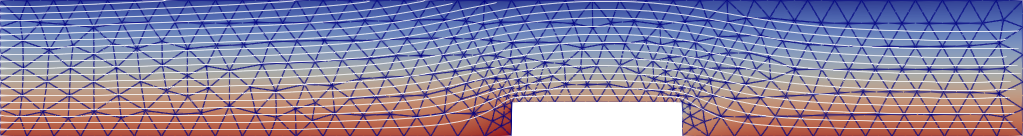
\includegraphics[width=\textwidth,angle=-5.7296]{stepflowlin}  % 0.1 radian = 5.7296 degrees
\caption{(FIXME: PUT NEW CODE RESULT)  A 2D glacier flowing over a bedrock step.  Arrows show velocity $\bu$ and shading is by pressure $p$.}
\label{fig:glacier:bedstep}
\end{figure}

\section{Glen-Stokes model} \label{sec:stokes}

Let us start from the Glen-Stokes model for ice dynamics.  This model, also covered in \cite{GreveBlatter2009,JouvetRappaz2011}, applies on any 2D or 3D domain $\Omega$ which has a piecewise smooth boundary.  Allowing any Glen exponent $n\ge 1$, the equations are:
\begin{align}
- \nabla \cdot \tau + \nabla p &= \rho \bg &&\text{\emph{stress balance}} \label{forcebalance} \\
\nabla \cdot \bu &= 0 &&\text{\emph{incompressibility}} \label{incompressible} \\
D\bu &= A_n |\tau|^{n-1} \tau &&\text{\emph{Glen flow law}} \label{flowlaw}
\end{align}
The notation here generally follows my notes and slides, including velocity $\bu$, pressure $p$, ice density $\rho$, acceleration of gravity $\bg$, deviatoric stress tensor $\tau$, strain rate tensor $D\bu$, and ice softness $A_n$.  A key idea is that tensors $D\bu$ and $\tau$ are symmetric (conservation of angular momentum) and have trace zero (incompressibility).  Note that $D\bu$ is the symmetric part of the velocity derivative tensor $\grad \bu$:
\begin{equation}
(D\bu)_{ij} = \frac{1}{2} \left(\grad\bu + \grad\bu^\top\right) = \frac{1}{2} \left((u_i)_{x_j} + (u_j)_{x_i}\right) \label{strainrate}
\end{equation}
The full (Cauchy) stress tensor $\sigma$ is the deviatoric stress tensor $\tau$ minus the pressure,
\begin{equation}
    \sigma = \tau - p\,I,  \label{cauchystress}
\end{equation}
so equation \eqref{forcebalance} simply says $-\Div \sigma = \rho \bg$.  One may derive from \eqref{cauchystress} that $p = -\frac{1}{2} \trace \sigma$ (in 2D), thus the pressure is the negative of the average normal stress.  By definition $\Div\tau$ in \eqref{forcebalance} is a vector with components which are the divergences of the columns:
\begin{equation}
    \left(\nabla \cdot \tau\right)_i = \left(\tau_{1i}\right)_{x_1} + \left(\tau_{2i}\right)_{x_2}  \label{divtaudefn}
\end{equation}
Note $\nabla\cdot \tau$, $\nabla p$, and $\bg$ are regarded as column vectors.

The viscosity form of \eqref{flowlaw} can also be found in the notes:
\begin{equation}
\tau = 2\nu D\bu = B_n |D\bu|^{\frac{1}{n} - 1} D\bu  \label{viscflowlaw}
\end{equation}
Here $B_n = (A_n)^{-1/n}$ is the ice hardness in units $\text{Pa}\,\text{s}^{1/n}$.  The tensor norm notation used in \eqref{flowlaw}  and \eqref{viscflowlaw} is defined as follows, with the summation convention:
\begin{align*}
|\tau|^2 = \frac{1}{2} \trace\left(\tau^2\right) = \frac{1}{2} \tau_{ij} \tau_{ij}, \qquad |D\bu|^2 = \frac{1}{2} \trace\left((D\bu)^2\right) = \frac{1}{2} (D\bu)_{ij} (D\bu)_{ij}
\end{align*}
Using \eqref{viscflowlaw} we can eliminate $\tau$ from equation \eqref{forcebalance}, thereby rewriting the system in terms of velocity $\bu$ and pressure $p$ only:
\begin{align}
- \nabla \cdot \left(B_n |D\bu|^{\frac{1}{n} - 1} D\bu\right) + \nabla p &= \rho \mathbf{g} \label{stokes} \\
\Div \bu &= 0 \label{incompagain}
\end{align}

From now on we denote the points of the 2D region $\Omega$ by $(x,z)$, and we add an angle parameter: gravity is at an angle $\alpha$ with the $z$-direction, so that $\bg = \left<g\sin\alpha,-g\cos\alpha\right>$ where $g>0$.  The numerical model in these notes solves system \eqref{stokes}, \eqref{incompagain} with a body force given by this $\rho \bg$.  A solution of the problem is a pair $(\bu,p)$.

Certain glacier-suitable velocity and stress boundary conditions will be used here.  We assume that base, top, inflow, and outflow boundaries can all be identified.  On the base we require no slip:
\begin{align}
\bu &= 0  &&\text{\emph{base}} \label{basebc} \\
\intertext{(Modifying this is not too difficult, and is an excellent exercise.)  On the top we set a condition of zero applied stress, $\sigma\hbn=0$:}
\left(B_n |D\bu|^{\frac{1}{n} - 1} D\bu - pI\right) \hbn &= 0  &&\text{\emph{top}} \label{topbc} \\
\intertext{The inflow boundary is the left side, which has outward normal $\hbn=\left<-1,0\right>$, and here we set a nonzero inflow velocity:}
\bu &= \left<f(z),0\right>  &&\text{\emph{inflow}} \label{inflowbc} \\
\intertext{The implemented function $f(z)$ satisfies the slab-on-slope equations for a given thickness $H_{\text{in}}$; see below.  On the outflow boundary, which is the right side and has $\hbn=\left<1,0\right>$ in the implemented form, we set a nonzero hydrostatic normal stress using the ice thickness $H_{\text{out}}$ at that location:}
\left(B_n |D\bu|^{\frac{1}{n} - 1} D\bu - pI\right) \hbn &= \big<- \rho g \cos\alpha (H_{\text{out}}-z),  \notag && \\
    &\qquad\quad \rho g\sin\alpha (H_{\text{out}}-z)\big> && \text{\emph{outflow}} \label{outflowbc}
\end{align}


\section{Slab-on-slope solutions}  \label{sec:slab}

Testing a numerical model requires verification tools, namely exact solutions.  Such solutions are in short supply for the Glen-Stokes model, so now we recapitulate the slab-on-slope construction given in the notes, allowing any Glen exponent $n$.  This also generates inflow and outflow boundary conditions which can be used for more general flows.

Using component notation for 2D, equations \eqref{stokes}, \eqref{incompagain} become the following Glen-Stokes model in coordinates $(x,z)$ and velocity components $\bu=\left<u,w\right>$:
\begin{align}
- \left(B_n |D\bu|^{\frac{1}{n}-1} u_x\right)_x - \left(\frac{1}{2} B_n |D\bu|^{\frac{1}{n}-1} \left(u_z+w_x\right)\right)_z + p_x &= \rho g\sin\alpha \label{planestressx} \\
- \left(\frac{1}{2} B_n |D\bu|^{\frac{1}{n}-1} \left(u_z+w_x\right)\right)_x - \left(B_n |D\bu|^{\frac{1}{n}-1} w_z\right)_z + p_z &= -\rho g\cos\alpha \label{planestressz} \\
u_x + w_z &= 0 \label{planeincomp}
\end{align}
The strain-rate norm expands to
\begin{equation}
    |D\bu|^2 = \frac{1}{2} \left(u_x^2 + \frac{1}{2}(u_z+w_x)^2 + w_z^2\right)  \label{planeDnorm}
\end{equation}

Consider either an infinitely-long or a periodic slab flow.  It has fixed ($x$-independent) values of the bed elevation $b$ and the surface elevation $h$, so the domain is $\Omega = \{(x,z)\,|\,b < z < h\}$.  Assume that the boundary stresses are also $x$-independent.  Then there is no variation in $x$, i.e.~$\partial/\partial x=0$, so the system simplifies:
\begin{align}
- \left(\frac{1}{2}B_n |D\bu|^{\frac{1}{n}-1} u_z\right)_z &= \rho g\sin\alpha \label{slabstresses} \\
p_z &= -\rho g\cos\alpha \notag \\
w_z &= 0 \notag
\end{align}
Also, the strain-rate norm simplifies to $|D\bu| = \frac{1}{2} |u_z|$.  If we further assume that there is no melt or freeze at the base then $w=0$ identically; the ice velocity is bed and surface parallel.  Then an integration with respect to $z$, and assumption of zero pressure at the surface, yields hydrostatic pressure:
\begin{equation}
p(z) = \rho g\cos\alpha (h-z)  \label{pslab}
\end{equation}

Now \eqref{slabstresses} yields a single nontrivial equation for the horizontal velocity:
    $$- \left(\frac{B_n}{2^{1/n}} |u_z|^{\frac{1}{n}-1} u_z\right)_z = \rho g\sin\alpha$$
As we expect $u_z>0$, rearrangement gives
    $$\left((u_z)^{1/n} \right)_z = - \frac{2^{1/n} \rho g\sin\alpha}{B_n}$$
This can be vertically-integrated downward from the surface $z=h$, using the no-stress condition, which simplifies to $u_z=0$, to give
\begin{equation}
u_z = 2 \left(\frac{\rho g\sin\alpha}{B_n}\right)^n (h-z)^n  \label{uzslab}
\end{equation}
Integrating vertically again, upward from the base $z=b$ where $u=0$, gives
\begin{equation}
u(z) = \frac{2}{n+1} \left(\frac{\rho g\sin\alpha}{B_n}\right)^n \left((h-b)^{n+1} - (h-z)^{n+1}\right)  \label{uslab}
\end{equation}

Formulas \eqref{pslab} and \eqref{uslab} exactly solve the Stokes equations and the described boundary conditions.  They will be used for verifying the numerical solver.

Additionally these slab-on-slope formulas allow us to set boundary conditions which lead to glaciologically-reasonable solutions for more general shapes like that shown in Figure \ref{fig:glacier:bedstep}.  In the implemented cases, the inflow side has \eqref{uslab} applied as a Dirichlet condition, as in \eqref{inflowbc}.  On the outflow side we apply a normal stress derived from \eqref{uzslab}.  That is, using the facts that $w=0$, $u_x=0$, $|D\bu| = \frac{1}{2} u_z$, and $\hbn=\left<1,0\right>$, we have
\begin{align*}
\sigma \hbn &= \left(B_n |D\bu|^{\frac{1}{n}-1} D\bu - pI\right)\hbn = \left(B_n |D\bu|^{\frac{1}{n}-1} \begin{pmatrix} u_x & \frac{1}{2}(u_z+w_x) \\ \frac{1}{2}(u_z+w_x) & w_z \end{pmatrix} - pI\right)\hbn \\
    &= B_n \left(\frac{1}{2} u_z\right)^{\frac{1}{n}-1} \begin{pmatrix} 0 \\ \frac{1}{2} u_z \end{pmatrix} - \begin{pmatrix} p \\ 0 \end{pmatrix} = \begin{pmatrix} - p \\ \frac{B_n}{2^{1/n}} (u_z)^{1/n} \end{pmatrix} = \begin{pmatrix} - \rho g\cos\alpha (h-z) \\ \rho g\sin\alpha (h-z) \end{pmatrix}
\end{align*}
This justifies formula \eqref{outflowbc}.


\section{Weak form} \label{sec:weakform}

Equations \eqref{stokes} and \eqref{incompagain} are called the \emph{strong form} of the model.  An integral equation form of the same equations, the \emph{weak form}, is needed when building a numerical finite element (FE) method \cite{Elmanetal2014}.  This new form is derived by multiplying the strong form equations by test functions and then integrating over $\Omega$.  This defines a nonlinear functional $F$, that is, a function which takes functions as input and returns scalars.  The weak form says that $F$ is zero when acting on test functions.  The significance of the weak form can be stated in several ways:
\begin{itemize}
\item It is well-posed in the sense of always having a unique solution  for glaciologically-relevant boundary values \cite{JouvetRappaz2011}.
\item It has a larger space of potential solutions than the strong form, for instance it is more flexible with respect to discontinuities in the data.
\item An FE method can create test functions, via local constructions which work on a mesh of triangles or quadrilaterals, and these go into the weak form.  This framework is more flexible with respect to problem geometry than are, for example, finite difference methods based on the strong form.
\end{itemize}

A solution to the weak form stated below is a pair $(\bu,p)$ wherein each function lives in a certain function space.  We write $\bu\in V_D$ and $p \in Q$ here, but the Sobolev spaces $V_D$ and $Q$ are precisely-identified in \cite{JouvetRappaz2011}.  Test functions $\bv\in V_0$ and $q\in Q$ come from nearly the same spaces, with $V_D$ and $V_0$ differing only by the value on the Dirichlet boundary: $\bu\in V_D$ satisfies a nonhomogeneous inflow condition \eqref{inflowbc} while $\bv\in V_0$ is zero there.

To give an initial definition of $F$ we multiply \eqref{stokes} by $\bv\in V_0$ and \eqref{incompagain} by $q\in Q$, then add and integrate:
\begin{equation}
F(\bu,p;\bv,q) = \int_\Omega - \left(\nabla \cdot \left(B_n |D\bu|^{\frac{1}{n} - 1} D\bu\right)\right)\cdot \bv + \nabla p \cdot \bv - \rho \mathbf{g} \cdot \bv - \left(\nabla \cdot \bu\right) q \label{nonfuncone}
\end{equation}
However, the desired definition of $F$ balances the number of derivatives on $(\bv,q)$ versus $(\bu,p)$, that is, it has only first derivatives on $\bu,\bv$, and no derivative on $p,q$.  To make this change we need integration-by-parts.

Recall the product rule $\nabla \cdot(f\bX) = \grad f\cdot \bX + f \nabla \cdot \bX$ and the divergence theorem $\int_\Omega \nabla \cdot (f\bX) = \int_{\partial \Omega} f\bX \cdot \hbn$.  Denoting $\tau = B_n |D\bu|^{\frac{1}{n} - 1} D\bu$ for convenience we have
\begin{align*}
\int_\Omega \left(\nabla \cdot \tau\right)\cdot \bv &= \sum_{j=1}^2 \int_\Omega \nabla \cdot (\tau_{j\circ})\, v_j = \sum_{j=1}^2 \int_\Omega \nabla \cdot (\tau_{j\circ} v_j) - \tau_{j\circ} \nabla v_j \\
  &= \sum_{j=1}^2 \int_{\partial \Omega} (\tau_{j\circ} v_j) \cdot \hbn - \int_\Omega \tau_{j\circ} \cdot \nabla v_j = \int_{\partial \Omega} (\tau \hbn)\cdot \bv - \int_\Omega \trace(\tau \nabla \bv)
\end{align*}
where $\circ$ denotes a vector entry index and $\tau_{j\circ}$ denotes the $j$th row of $\tau$.  Here $\grad\bv$ defines a $2\times 2$ matrix,
\newcommand{\treftwo}[2]{\left[\begin{array}{c|c} & \\ #1 & #2 \\ & \end{array}\right]}
\newcommand{\trefthree}[3]{\left[\begin{array}{c|c|c} & & \\ #1 & #2 & #3 \\ & & \end{array}\right]}
    $$\grad \bv = \treftwo{\grad v_1}{\grad v_2} = \begin{bmatrix}
    (v_1)_{x_1} & (v_2)_{x_1} \\
    (v_1)_{x_2} & (v_2)_{x_2}
    \end{bmatrix}$$
and so
    $$\trace(\tau \grad \bv) = \sum_{j=1}^3 \tau_{j\circ} \cdot \grad v_j = \sum_{i,j=1}^3 \tau_{ji} (v_j)_{x_i}$$
(Some sources write $A:B$ for $\trace(AB)$ \cite{JouvetRappaz2011}.)  Note $\trace(\tau \grad \bv) = \trace(\tau D\bv)$ because $\trace(AB)=0$ if $A$ is symmetric and $B$ is antisymmetric.  (To show this take $A=\tau$ and $B=\grad\bv-D\bv$.)  Finally we do a straightforward integration-by-parts on the pressure part of $F$:
    $$\int_\Omega \nabla p \cdot \bv = \int_\Omega \nabla\cdot (p\,\bv) - p (\nabla \cdot \bv) = \int_{\partial \Omega} p\hbn \cdot \bv - \int_\Omega p (\nabla \cdot \bv)$$

The above facts allow us to rewrite \eqref{nonfuncone} with a normal stress boundary integral:
\begin{equation}
F(\bu,p;\bv,q) =  \int_\Omega \left[\trace(\tau D\bv) - p (\nabla \cdot \bv) - \left(\nabla \cdot \bu\right) q - \rho \mathbf{g} \cdot \bv\right] - \int_{\partial\Omega} (\sigma \hbn)\cdot \bv \label{nonfunctwo}
\end{equation}
(We have denoted $\sigma=\tau-pI$ for brevity.)  Note $\bu,\bv$ appear with first derivatives and $p,q$ have no derivatives.

Next recall that $\bv\in V_0$ satisfies $\bv=0$ along the base and inflow surfaces.  Thus these parts of the integral over $\partial\Omega$ in \eqref{nonfunctwo} are zero.  Conditions \eqref{topbc}, \eqref{outflowbc} now completely eliminate the unknown solution $\bu,p$ from the boundary integral.  The above computations yield our final formula for the nonlinear functional:
\begin{align}
F(\bu,p;\bv,q) &= \int_\Omega B_n |D\bu|^{\frac{1}{n} - 1} \trace(D\bu D\bv) - p (\nabla \cdot \bv) - \left(\nabla \cdot \bu\right) q \label{defineF} \\
    &\qquad  - \int_\Omega \rho \mathbf{g} \cdot \bv - \int_{\{\text{outflow}\}} C_{\text{out}} \rho g \cos\alpha (h-z) v  \notag
\end{align}

The weak form of the Glen-Stokes model is the statement that, at the solution $\bu\in V_D$ and $p\in Q$, functional $F$ in \eqref{defineF} is zero in all test function directions:
\begin{equation}
F(\bu,p;\bv,q) = 0 \qquad \text{ for all } \bv\in V_0 \text{ and } q\in Q  \label{weak}
\end{equation}
This weak formulation is proven in \cite[Theorem 3.8]{JouvetRappaz2011} to be well-posed, so that a unique solution exists.  The well-posedness theorem makes reasonable assumptions about the domain $\Omega$ and the boundary data, and these are satisfied in the cases we consider.  Noting that the last two integrals in \eqref{defineF} can be regarded as source terms for stress, if the inflow velocity is zero and if we replace the source terms by zero---we remove gravity and outflow stresses---then the unique solution to \eqref{weak} is $\bu=0$ and $p=0$.

Now our goal is to accurately approximate the solution $(\bu,p)$ of \eqref{weak} using an FE method.


\section{Finite element method} \label{sec:femethod}

This section gives a very abbreviated summary of our finite element (FE) method to solve the glaciological Glen-Stokes equations, but better coverage of FE methods, including for the linear Stokes equations, is in references \cite{Braess2007,Bueler2021,Elmanetal2014}.  The method here uses Firedrake \cite{Rathgeberetal2016}; we do \emph{not} implement most of the following techniques ourselves.

The fundamental FE idea is to replace the infinite-dimensional function spaces appearing in the weak form \eqref{weak} with finite-dimensional subspaces constructed locally from triangles (or quadrilaterals) in a mesh.  The approximate solution $(\bu^h,p^h)$ lives in these subspaces, and the functional $F$ in \eqref{defineF} is computed on test functions from these subspaces.  Requiring $F$ to be zero over a basis of the test-functions, as stated in equation \eqref{feweak} below, defines the (nonlinear) discrete equations.  We solve this nonlinear system of algebraic equations using Newton's method \cite{Bueler2021}.

The mesh itself is denoted $\mathcal{T}_h$.  It covers the domain $\Omega$ by a finite set of $K$ non-overlapping open elements\footnote{Here elements are either triangles or quadrilaterals, but we stick with notation $\mathcal{T}_h$ and $\triangle_k$.} $\triangle_k$, is stored in a \texttt{.msh} file generated by Gmsh; see section \ref{sec:implementation} below.  The subscript ``$h$'' on $\mathcal{T}_h$ also denotes the maximum diameter of the triangles.  Let $N_1$ be the number of element nodes (vertices) in the mesh, including nodes on $\partial\Omega$, and denote the coordinates of the $i$th node by $(x_i,z_i)$ for $i=0,1,\dots,N_1-1$.

For a triangle $\triangle_k$ there are various choices of a \emph{finite element space}, a space of low-degree polynomials defined on that triangle.  By default we use two particular FE spaces, denoted $P_1$ for the pressure and $(P_2)^2$ for velocity.  Using such paired spaces is called a \emph{mixed method}, and $P_2$-$P_1$ chosen here are the lowest-order \emph{Taylor-Hood} elements \cite{Elmanetal2014}.

Consider just one triangle.  The name $P_1$ refers to the space of linear functions $a + b x + c z$ on the triangle.  The three vertices of the triangle are the preferred degrees of freedom (Figure \ref{fig:fedofs} left) in the sense that any $P_1$ function on the triangle is determined by its values at these vertices.  The $P_2$ space, used for the scalar components of velocity, is the space of quadratic functions $a + bx + cy + dx^2 + exy + fy^2$, with six degrees of freedom at the vertices and edge midpoints (Figure \ref{fig:fedofs} right).  The function spaces for quadrilaterals are comparable \cite{Elmanetal2014}, but we omit the details.

\begin{figure}[ht]
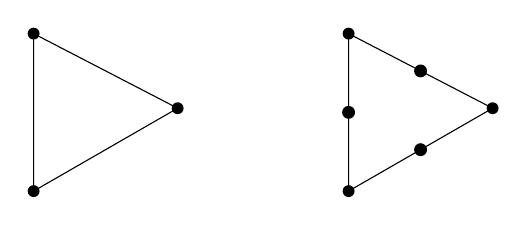
\begin{tikzpicture}[scale=1.0,dot/.style={draw,circle,fill=black,inner sep=1.5pt,pos=0.5}]
\newcommand{\ldot}{node[circle,fill=black,inner sep=0.5pt] (0.0pt) {.}}
\pgfmathsetmacro{\xo}{0.0}
\pgfmathsetmacro{\yo}{0.0}
  \draw[black] (0.000000+\xo,-2.000000+\yo) \ldot -- (1.828947+\xo,-0.947368+\yo) \ldot -- (0.000000+\xo,0.000000+\yo) \ldot -- (0.000000+\xo,-2.000000+\yo) ;
\pgfmathsetmacro{\xo}{4.0}
  \draw[black] (0.000000+\xo,-2.000000+\yo) \ldot -- node[dot](){}  (1.828947+\xo,-0.947368+\yo) \ldot -- node[dot](){} (0.000000+\xo,0.000000+\yo) \ldot -- node[dot](){} (0.000000+\xo,-2.000000+\yo) ;
\end{tikzpicture}
\caption{$P_1$ and $P_2$ triangular elements.}
\label{fig:fedofs}
\end{figure}

A continuous scalar function on $\Omega$ which is piecewise-linear on each triangle, i.e.~in $P_1$ on each triangle, is determined by its values at the $N_1$ nodes of the mesh.  The space of such functions is a finite-dimensional subspace $Q^h \subset Q$ of the pressure space $Q$ used in the weak form \eqref{weak}.  Next, a continuous scalar function on $\Omega$ which is piecewise-quadratic ($P_2$) on each triangle is determined by its values at the nodes \emph{and} edge midpoints in the mesh \cite{Elmanetal2014}.  Let $N_2$ denote the number of all such $P_2$ degrees of freedom, not including Dirichlet boundary nodes.  A small example of this kind of mesh is shown in Figure \ref{fig:fedims}.

\begin{figure}[ht]
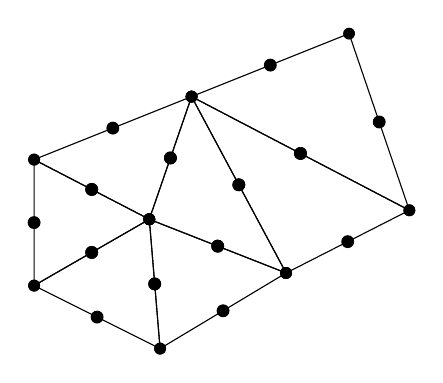
\begin{tikzpicture}[scale=0.8,dot/.style={draw,circle,fill=black,inner sep=1.5pt,pos=0.5}]
\pgfmathsetmacro{\xo}{0.0}
\pgfmathsetmacro{\yo}{0.0}
\newcommand{\ldot}{node[circle,fill=black,inner sep=0.5pt] (0.0pt) {.}}
  \draw[black] (0.000000+\xo,-2.000000+\yo) \ldot -- node[dot](){}  (1.828947+\xo,-0.947368+\yo) \ldot -- node[dot](){} (0.000000+\xo,0.000000+\yo) \ldot -- node[dot](){} (0.000000+\xo,-2.000000+\yo) ;
  \draw[black] (2.000000+\xo,-3.000000+\yo) \ldot -- node[dot](){} (1.828947+\xo,-0.947368+\yo) \ldot -- node[dot](){} (0.000000+\xo,-2.000000+\yo) \ldot -- node[dot](){} (2.000000+\xo,-3.000000+\yo) ;
  \draw[black] (0.000000+\xo,0.000000+\yo) \ldot -- node[dot](){} (1.828947+\xo,-0.947368+\yo) \ldot -- node[dot](){} (2.500000+\xo,1.000000+\yo) \ldot -- node[dot](){} (0.000000+\xo,0.000000+\yo) ;
  \draw[black] (1.828947+\xo,-0.947368+\yo) \ldot -- node[dot](){} (2.000000+\xo,-3.000000+\yo) \ldot -- node[dot](){} (4.000000+\xo,-1.799890+\yo) \ldot -- node[dot](){} (1.828947+\xo,-0.947368+\yo) ;
  \draw[black] (4.000000+\xo,-1.799890+\yo) \ldot -- node[dot](){} (5.957182+\xo,-0.804788+\yo) \ldot -- node[dot](){} (2.500000+\xo,1.000000+\yo) \ldot -- node[dot](){} (4.000000+\xo,-1.799890+\yo) ;
  \draw[black] (2.500000+\xo,1.000000+\yo) \ldot -- node[dot](){} (1.828947+\xo,-0.947368+\yo) \ldot -- node[dot](){} (4.000000+\xo,-1.799890+\yo) \ldot -- node[dot](){} (2.500000+\xo,1.000000+\yo) ;
  \draw[black] (2.500000+\xo,1.000000+\yo) \ldot -- node[dot](){} (5.957182+\xo,-0.804788+\yo) \ldot -- node[dot](){} (5.000000+\xo,2.000000+\yo) \ldot -- node[dot](){} (2.500000+\xo,1.000000+\yo) ;
\end{tikzpicture}

\caption{A mesh with $K=7$ triangular elements, $N_1=8$ $P_1$ degrees of freedom (nodes), and $N_2=22$ degrees of freedom for $P_2$.}
\label{fig:fedims}
\end{figure}

However, velocity fields are vector-valued.  Let us define $V_0^h$ to be the space of \emph{pairs} of scalar piecewise-quadratic functions on $\Omega$, additionally requiring them to be zero on the base and inflow (i.e.~Dirichlet) boundaries, where \eqref{basebc} and \eqref{inflowbc} apply.  The functions in $V_0^h$ are 2D vector fields with components which are piecewise-quadratic scalar functions in $P_2$.  We define $V_D^h$ to be the nearly the same space except satisfying \eqref{inflowbc} on the inflow boundary.  There are two $P_2$ subspaces used in the FE weak form \eqref{feweak} below: $V_0^h \subset V_0$, $V_D^h \subset V_D$.

Finally we think about the test functions, specifically the basis functions called \emph{hat functions},\footnote{Figure 1.6 in \cite{Elmanetal2014} and Figure 10.4 in \cite{Bueler2021} show $P_1$ hat functions, while Figure 1.7 in \cite{Elmanetal2014} suggests how $P_2$ hat functions would look.} used in the FE weak form \eqref{feweak}.  For pressure, let $\psi_j(x,z)$ be a $P_1$ hat function from $Q^h$ which is linear on each triangle, continuous on $\Omega$, equal to one at node $(x_j,z_j)$, and otherwise zero at all other nodes.  Thus $\psi_j(x_i,z_i) = \delta_{ij}$.  The set $\{\psi_j\}$ is a set of $N_1$ linearly-independent functions in $Q^h$, and thus a basis of $Q^h$.  Similarly, for every $P_2$ node which is not in the base or inflow boundary, whether a triangle vertex or edge midpoint, there is a $P_2$ hat function.  Pairs of such piecewise-quadratic hat functions, $(\phi_j(x,z),0)$ or $(0,\phi_j(x,z))$, form a basis of $2N_2$ functions for the velocity test space $V_0^h$.

When using $P_2$ elements for velocity and $P_1$ elements for pressure we see that the dimension of the velocity space is much higher than the pressure space.  For example, for the $N_1=356$ vertex mesh shown in Figure \ref{fig:glacier:bedstep}, the velocity dimension $2N_2=2646$ is seven times greater than $N_1$.  Such a dimension imbalance turns out to be desirable!  As explained in the FE literature under the obscure name ``inf-sup condition'' \cite{Braess2007,Bueler2021,Elmanetal2014}, Stokes equations mixed methods are only stable if the velocity space is sufficiently-large relative to the pressure space.

Finally we can state the FE method itself.  It is a finite-dimensional approximation of weak form \eqref{weak}, namely it finds $\bu^h \in V_D^h$ and $p^h \in Q^h$ so that
\begin{equation}
F(\bu^h,p^h;\bv^h,q^h) = 0 \qquad \text{ for all } \bv^h\in V_0^h \text{ and } q^h\in Q^h  \label{feweak}
\end{equation}
Note that relative to \eqref{weak} the nonlinear functional $F$ is unchanged and we have merely added ``$h$'' superscripts to all continuum quantities!  Problem \eqref{feweak} can be shown to be well-posed by the same theory that applies to the continuum problem \cite[Theorem 4.3]{JouvetRappaz2011}.

By linearity of $F$ in the $\bv,q$ positions, it suffices to consider only a basis of test functions, i.e.~hat functions, from $V_0^h$ and $Q^h$.  However, \eqref{feweak} is a nonlinear system which should be solved by Newton's method \cite{Bueler2021,Kelley2003}.  In fact, suppose we have some current iterate $\bu^h,p^h$ which does not exactly solve \eqref{feweak}.  Then for each test function $\bv^h$ or $q^h$, i.e.~for each hat function, the value of the ``residual'' $F(\bu^h,p^h;\bv^h,q^h)$ can be computed concretely, though also approximately, by quadrature \cite{Bueler2021,Elmanetal2014}.  Also we can use the current iterate, and the derivatives of $F$, to evaluate the Jacobian at the current iterate.  This ``assembly'' process generates a system of sparse, linear algebraic equations, namely the Newton step equations of the discrete Glen-Stokes problem.  In actuality the equations are assembled element-by-element, not node-by-node, in the sense that for each triangle $\triangle_k$ the contribution from that triangle is added to the correct equation, but this represents an unneeded detail.  The point of using an FE library like Firedrake is that it hides the assembly process and it allows us to think about the problem at a higher level \cite{Rathgeberetal2016}.

At each Newton step we solve a sparse and indefinite linear system.  These systems have a well-known block structure (Figure \ref{fig:lowspy}), so we may apply a Schur complement preconditioner in a GMRES Krylov iteration \cite{Elmanetal2014,GolubVanLoan2013}.  This buzzword salad suggests the complexity of solver technology, and we abandon further explanation, but see Chapter 14 of \cite{Bueler2021}.

\begin{figure}[h]
\includegraphics[width=0.45\textwidth]{lowspy}
%./domain.py -hmesh 300.0 -refine_corner 2 -o low.geo
%gmsh -2 low.geo
%./flow.py -mesh low.msh -s_mat_type aij -s_ksp_view_mat :low.m:ascii_matlab
% then spy() in Matlab
\caption{Sparsity pattern of the Newton step linear system, when solving the Stokes equations on a coarse mesh ($K=52,N_1=40,N_2=131$).}
\label{fig:lowspy}
\end{figure}


\section{Implementation in Python} \label{sec:implementation}

This section gives a practical view of our codes, including how they are divided into modules and the sequence in which they are used in practice.  In overview, we implement problem \eqref{feweak}, and make the stated discretization choices, in Python using Firedrake \cite{Rathgeberetal2016}.  The PETSc solver library \cite{Balayetal2018,Bueler2021} is called via Firedrake on the discretized nonlinear equations.

To define the nonlinear residual function $F$ in \eqref{defineF}, the UFL domain-specific language, designed for describing such weak forms \cite{Alnaesetal2014}, is applied.  This language comes rather close to the mathematical form.  Compare \eqref{strainrate}, \eqref{viscflowlaw}, and \eqref{defineF} to the code as written:
\begin{Verbatim}[fontsize=\small,frame=lines]
def D(U):
    return 0.5 * (grad(U) + grad(U).T)
Du2 = 0.5 * inner(D(u), D(u)) + (eps * Dtyp)**2.0
rr = 1.0/3.0 - 1.0
F = ( inner(B3 * Du2**(rr/2.0) * D(u), D(v)) - p * div(v) - div(u) * q ) * dx \
    - inner(f_body, v) ) * dx - inner(outflow_sigma, v) * ds(bdryids['outflow'])
\end{Verbatim}
Firedrake knows how to take this code, plus a choice of mesh and function spaces, and run the assemble process to create the Newton step equations for this problem.  Then Firedrake's \texttt{solve()} command solves \eqref{feweak} \cite{Rathgeberetal2016}.

\medskip
As shown in Figure \ref{fig:blockdiagram} there are three major Python components:
\begin{itemize}
\item \texttt{domain.py}: \quad  This writes an outline of the domain $\Omega$ into an ASCII file (\texttt{.geo} extension) using the Gmsh \cite{GeuzaineRemacle2009} geometry description language.  Note Gmsh can be used to examine and mesh this domain interactively, or at the command-line as above.  Portions of the boundary are marked with integer tags; see the Python dictionary \texttt{bdryids}.

\item \texttt{momentummodel.py}: \quad  Implements \texttt{class MomentumModel}.  Most actual ice physics is isolated here, including physical constants and the Stokes problem weak form \eqref{defineF}.  The \texttt{solve()} method assembles and solves the nonlinear Glen-Stokes problem \eqref{weak} using Firedrake's \texttt{solve()} command.  This solver has option prefix \texttt{s\_}.

\item \texttt{flow.py}: \quad  This driver reads user options, loads the mesh from a Gmsh \texttt{.msh} file, uses a \texttt{MomentumModel} object to solve the Stokes problem, and writes the solution into a Paraview-readable \texttt{.pvd} file.
\end{itemize}

\begin{figure}[h]
\bigskip
\tikzstyle{tool} = [draw, minimum size=2em]
\tikzstyle{module} = [draw, dashed, minimum size=2em]
\tikzstyle{other} = [draw, minimum size=2em, rounded corners=0.2cm]
\begin{tikzpicture}[node distance=3.8cm,>=latex]
    \node [tool]   (domain) {\texttt{domain.py}};
    \node [other]  (gmsh)[right of= domain] {Gmsh};
    \node [tool]   (flow)[right of=gmsh] {\texttt{flow.py}};
    \node [other]  (paraview)[right of=flow] {Paraview};
    \node [module] (momentummodel)[above left of=flow] {\begin{minipage}{4.0cm} \texttt{momentummodel.py} \footnotesize (\texttt{class MomentumModule}) \end{minipage}};
    \path[->] (domain) edge node[below] {\texttt{.geo}} (gmsh) ;
    \path[->] (gmsh) edge node[below] {\texttt{.msh}} (flow) ;
    \path[->] (flow) edge node[below] {\texttt{.pvd}} (paraview) ;
    \path[->] (momentummodel) edge[dashed] node {} ([xshift=-0.2cm]flow.north) ;
\end{tikzpicture}

\medskip
\caption{Users interact with the solid-outline tools in the given order.}
\label{fig:blockdiagram}
\end{figure}

Here is a simple example solving the default Stokes problem:

\medskip
\begin{Verbatim}
$ ./domain.py -o glacier.geo                   # create domain outline
$ gmsh -2 glacier.geo                          # mesh domain
$ source ~/firedrake/bin/activate              # start Firedrake
(firedrake) $ ./flow.py -mesh glacier.msh      # solve Stokes problem
(firedrake) $ paraview glacier.pvd             # visualize results
\end{Verbatim}
%$

\medskip
\noindent The \verb|README.md| file documents usage and regression testing more thoroughly.


\small

\bigskip
\bibliography{doc}
\bibliographystyle{siam}

\end{document}
